\documentclass[12pt,a4paper]{article}
\usepackage{ctex}
\title{基于YOLOv5模型的目标检测实验报告}
\author{}

\usepackage{hyperref}
\hypersetup{colorlinks=true, linkcolor=blue, anchorcolor=green, citecolor=green}
\usepackage{bm}
\usepackage{amssymb, amsmath, amsthm}
\usepackage{graphicx}
\usepackage{float}
\usepackage{booktabs}
\usepackage{multirow}
\usepackage{subcaption}
\usepackage{listings}
\usepackage{xcolor}
\usepackage{enumitem}

\lstset{
    language=Python,
    basicstyle=\ttfamily\small,
    keywordstyle=\color{blue},
    commentstyle=\color{gray},
    stringstyle=\color{red},
    breaklines=true,
    frame=single,
    numbers=left,
    numberstyle=\tiny\color{gray}
}

\begin{document}

\begin{titlepage}
    \centering
    \vspace*{1cm}
    
\includegraphics[width=0.6\textwidth]{ucas_logo.pdf}
    \vspace{1cm}

    {\Huge\bfseries 深度学习作业5\par}
    \vspace{1cm}
    {\LARGE 基于YOLOv5模型的目标检测实验\par}
    \vspace{3cm}

    \begin{tabular}{rl}
        {\kaishu\Large 成员：} & {\kaishu\Large \underline{\makebox[6cm]{202528014629014 刘浩}}} \\[0.8cm]
         & {\kaishu\Large \underline{\makebox[6cm]{202528014629012 雷夕入}}} \\[0.8cm]
         & {\kaishu\Large \underline{\makebox[6cm]{202528014629015 刘宇坤}}} \\[0.8cm]
        {\kaishu\Large 院所：} & {\kaishu\Large \underline{\makebox[6cm]{人工智能学院}}} \\[0.8cm]
    \end{tabular}

    \vfill

    {\large \today\par}
\end{titlepage}

\newpage
\tableofcontents
\newpage

% ==============================================================
\section{实验目的}
% ==============================================================

\begin{enumerate}
    \item 理解YOLOv5模型的基本原理和工作机制，包括单阶段检测框架、anchor-based预测方式和多尺度特征融合策略。
    \item 掌握YOLOv5模型的部署和使用方法，基于PyTorch和Ultralytics框架完成从数据准备、模型训练到推理评估的完整流程。
    \item 在自定义数据集（COCO128）上进行训练和评估，实现测试集检测精度（mAP@0.5）达到90\%以上。
    \item 通过分析训练过程中各损失分量（box、cls、dfl）的变化趋势，深入理解目标检测任务中定位、分类和分布预测三个子任务的联合优化过程。
\end{enumerate}

% ==============================================================
\section{实验原理}
% ==============================================================

\subsection{单阶段目标检测框架}

与两阶段检测器（如Faster R-CNN先生成候选区域、再分类回归）不同，YOLO（You Only Look Once）系列算法将目标检测建模为一个端到端的回归问题：将输入图像划分为$S \times S$的网格，每个网格单元直接预测边界框坐标和类别概率。YOLOv5采用anchor-based的检测方式，在每个网格单元预设多个不同尺寸和宽高比的锚框，网络学习预测相对于锚框的偏移量，而非从零开始回归绝对坐标。

对于每个预测框，网络输出包含中心点偏移$(t_x, t_y)$、宽高缩放$(t_w, t_h)$以及目标置信度$t_o$。最终的边界框坐标通过以下公式计算：
\begin{align}
b_x &= \sigma(t_x) + c_x \\
b_y &= \sigma(t_y) + c_y \\
b_w &= p_w \cdot e^{t_w} \\
b_h &= p_h \cdot e^{t_h}
\end{align}
其中$(c_x, c_y)$为网格单元的左上角坐标，$(p_w, p_h)$为锚框的宽高，$\sigma$为sigmoid函数，将中心偏移限制在$[0,1]$区间内。这种“锚框+偏移”的设计使得网络只需学习小幅度的修正量，大幅降低了回归难度。

\subsection{CSP-Darknet骨干网络}

YOLOv5采用CSP-Darknet53（Cross Stage Partial Darknet）作为骨干网络。CSP的核心思想是将特征图沿通道维度分为两路：一路经过密集残差块（C3模块）提取深层特征，另一路通过跳跃连接直接传递，最终将两路特征拼接融合。这种设计有两个关键优势：（1）减少了约50\%的计算量，因为只有一半的特征图需要通过计算密集的残差块；（2）保持了丰富的梯度流动路径，避免了深层网络中梯度消失的问题。

\subsection{FPN-PAN颈部网络}

为了有效检测不同尺度的目标，YOLOv5采用特征金字塔网络（FPN）与路径聚合网络（PAN）相结合的颈部结构。FPN通过自顶向下的路径将高层语义信息传递给低层特征图——高层特征"知道"图像中有什么（语义），但不精确"知道"在哪里（定位）；低层特征则相反。FPN的上采样+拼接操作将两者融合。PAN在此基础上增加了自底向上的路径，将低层精确的定位信息回传给高层，形成双向特征融合。

最终，检测在三个尺度的特征图上进行：
\begin{itemize}[leftmargin=*]
    \item $80 \times 80$特征图（$8\times$下采样）：负责检测小目标
    \item $40 \times 40$特征图（$16\times$下采样）：负责检测中等目标
    \item $20 \times 20$特征图（$32\times$下采样）：负责检测大目标
\end{itemize}

\subsection{损失函数}

YOLOv5的总损失由三个分量组成：
\begin{equation}
\mathcal{L}_{total} = \lambda_{box}\mathcal{L}_{box} + \lambda_{obj}\mathcal{L}_{obj} + \lambda_{cls}\mathcal{L}_{cls}
\end{equation}

边界框回归损失$\mathcal{L}_{box}$采用CIoU（Complete IoU）损失。CIoU在IoU的基础上同时考虑了三个几何因素：
\begin{equation}
\mathcal{L}_{CIoU} = 1 - IoU + \frac{\rho^2(\mathbf{b}, \mathbf{b}^{gt})}{c^2} + \alpha v
\end{equation}
其中$\rho^2$为预测框与真实框中心点的欧氏距离，$c$为最小外接矩形的对角线长度，$v$衡量宽高比的一致性，$\alpha$为权衡系数。相比IoU损失（不相交时梯度为零）和GIoU损失（收敛慢），CIoU同时优化重叠面积、中心距离和宽高比，收敛更快更稳定。

目标置信度损失$\mathcal{L}_{obj}$和分类损失$\mathcal{L}_{cls}$均使用二元交叉熵（BCE）损失，后者采用多标签形式以支持同一目标属于多个类别的情况。

% ==============================================================
\section{数据集分析}
% ==============================================================

COCO128是COCO数据集的一个微型子集，包含128张图像，涵盖80个目标类别，共标注了929个目标实例（平均每张图像约7.3个目标）。尽管数据规模极小，但图像内容丰富多样，包含行人、车辆、动物、家具、餐具等日常物体。

该数据集具有两个显著特点：

（1）目标尺度分布广泛：从占据图像大部分面积的公交车、卡车，到仅有数十像素的手机、领带，尺度跨度极大。这对模型的多尺度检测能力提出了严峻要求——如果仅在单一尺度上检测，大量小目标将被遗漏。

（2）类别分布不均匀："person"类别的实例数远多于其他类别（如"toothbrush""hair drier"等可能仅有1-2个实例）。这意味着模型对高频类别的学习更加充分，而低频类别的检测性能可能受限于样本不足。

在训练前，YOLOv5自动对数据集进行锚框聚类分析，利用k-means算法根据标注框的宽高分布确定9个锚框尺寸（3个尺度$\times$3个宽高比），确保锚框与目标尺度分布相匹配。

% ==============================================================
\section{模型设计与实现}
% ==============================================================

\subsection{网络架构}

本实验采用YOLOv5s（Small）作为检测模型，这是YOLOv5系列中最轻量的版本。根据训练日志，模型共包含154层、9153152个参数（约9.15M），计算量为24.2 GFLOPs。网络结构如表\ref{tab:arch}所示。

\begin{table}[H]
\centering
\caption{YOLOv5s网络架构（关键层）}
\label{tab:arch}
\begin{tabular}{clcc}
\toprule
\textbf{层编号} & \textbf{模块} & \textbf{输出通道} & \textbf{参数量} \\
\midrule
0 & Conv (k=6, s=2) & 32 & 3.5K \\
1 & Conv (k=3, s=2) & 64 & 18.6K \\
2 & C3 ($\times$1) & 64 & 18.8K \\
3 & Conv (k=3, s=2) & 128 & 74.0K \\
4 & C3 ($\times$2) & 128 & 115.7K \\
5 & Conv (k=3, s=2) & 256 & 295.4K \\
6 & C3 ($\times$3) & 256 & 625.2K \\
7 & Conv (k=3, s=2) & 512 & 1180.7K \\
8 & C3 ($\times$1) & 512 & 1182.7K \\
9 & SPPF (k=5) & 512 & 656.9K \\
\midrule
10--23 & FPN-PAN Neck & 128/256/512 & 2.83M \\
24 & Detect (3 heads) & 80 classes & 2.15M \\
\bottomrule
\end{tabular}
\end{table}

从参数分布来看，骨干网络（层0--9）占约4.17M参数（45.6\%），FPN-PAN颈部网络占约2.83M（30.9\%），检测头占约2.15M（23.5\%）。检测头的参数量较大是因为需要在三个尺度上分别输出$80+5$维的预测向量（80个类别概率 + 4个坐标偏移 + 1个目标置信度）。

\subsection{训练配置}

\begin{table}[H]
\centering
\caption{训练超参数配置}
\label{tab:config}
\begin{tabular}{ccc}
\toprule
\textbf{参数} & \textbf{配置} & \textbf{设计理由} \\
\midrule
优化器 & AdamW & 自适应学习率 + 解耦权重衰减 \\
初始学习率 & $1.19 \times 10^{-4}$ & Ultralytics自动选择 \\
动量 & 0.9 & Adam默认设置 \\
权重衰减 & $5 \times 10^{-4}$ & 正则化防止过拟合 \\
学习率调度 & 余弦退火 & 平滑衰减至接近零 \\
Warmup & 前3个epoch & 稳定训练初期梯度 \\
Batch size & 16 & GPU显存与训练稳定性的平衡 \\
训练轮次 & 50 epochs & 充分收敛 \\
输入尺寸 & $640 \times 640$ & YOLOv5标准输入尺寸 \\
AMP & 开启 & 混合精度加速训练 \\
\bottomrule
\end{tabular}
\end{table}

优化器选择：Ultralytics框架在\texttt{optimizer=auto}模式下自动选择了AdamW而非传统的SGD。AdamW将权重衰减从梯度更新中解耦，避免了Adam中L2正则化与自适应学习率之间的冲突，在小数据集上通常能更快收敛。

\subsection{数据增强策略}

COCO128仅有128张图像，直接训练极易过拟合。YOLOv5通过多种数据增强策略来缓解这一问题：
\begin{itemize}[leftmargin=*]
    \item Mosaic增强：将4张训练图像随机缩放后拼接为一张$640\times640$的合成图像。这等效地将batch size扩大了4倍（每个batch实际"看到"$16\times4=64$张图像的内容），同时增加了小目标出现在图像边缘的概率。
    \item 随机仿射变换：包括平移（$\pm$10\%）、缩放（$\pm$50\%）和水平翻转（50\%概率），增加了目标的空间多样性。
    \item HSV颜色抖动：随机调整色调（$\pm$1.5\%）、饱和度（$\pm$70\%）和亮度（$\pm$40\%），增强模型对光照变化的鲁棒性。
    \item Close Mosaic：在最后10个epoch关闭Mosaic增强，使模型在最终阶段适应真实的单张图像分布。
\end{itemize}

% ==============================================================
\section{实验结果与分析}
% ==============================================================

\subsection{训练过程分析}

\subsubsection{三个损失分量的变化}

图\ref{fig:train_loss}展示了训练过程中三个损失分量的变化曲线。整体来看，三种损失在前10个epoch内快速下降，随后进入平稳收敛阶段，但各分量的下降幅度和收敛速度存在明显差异。

\begin{figure}[H]
\centering
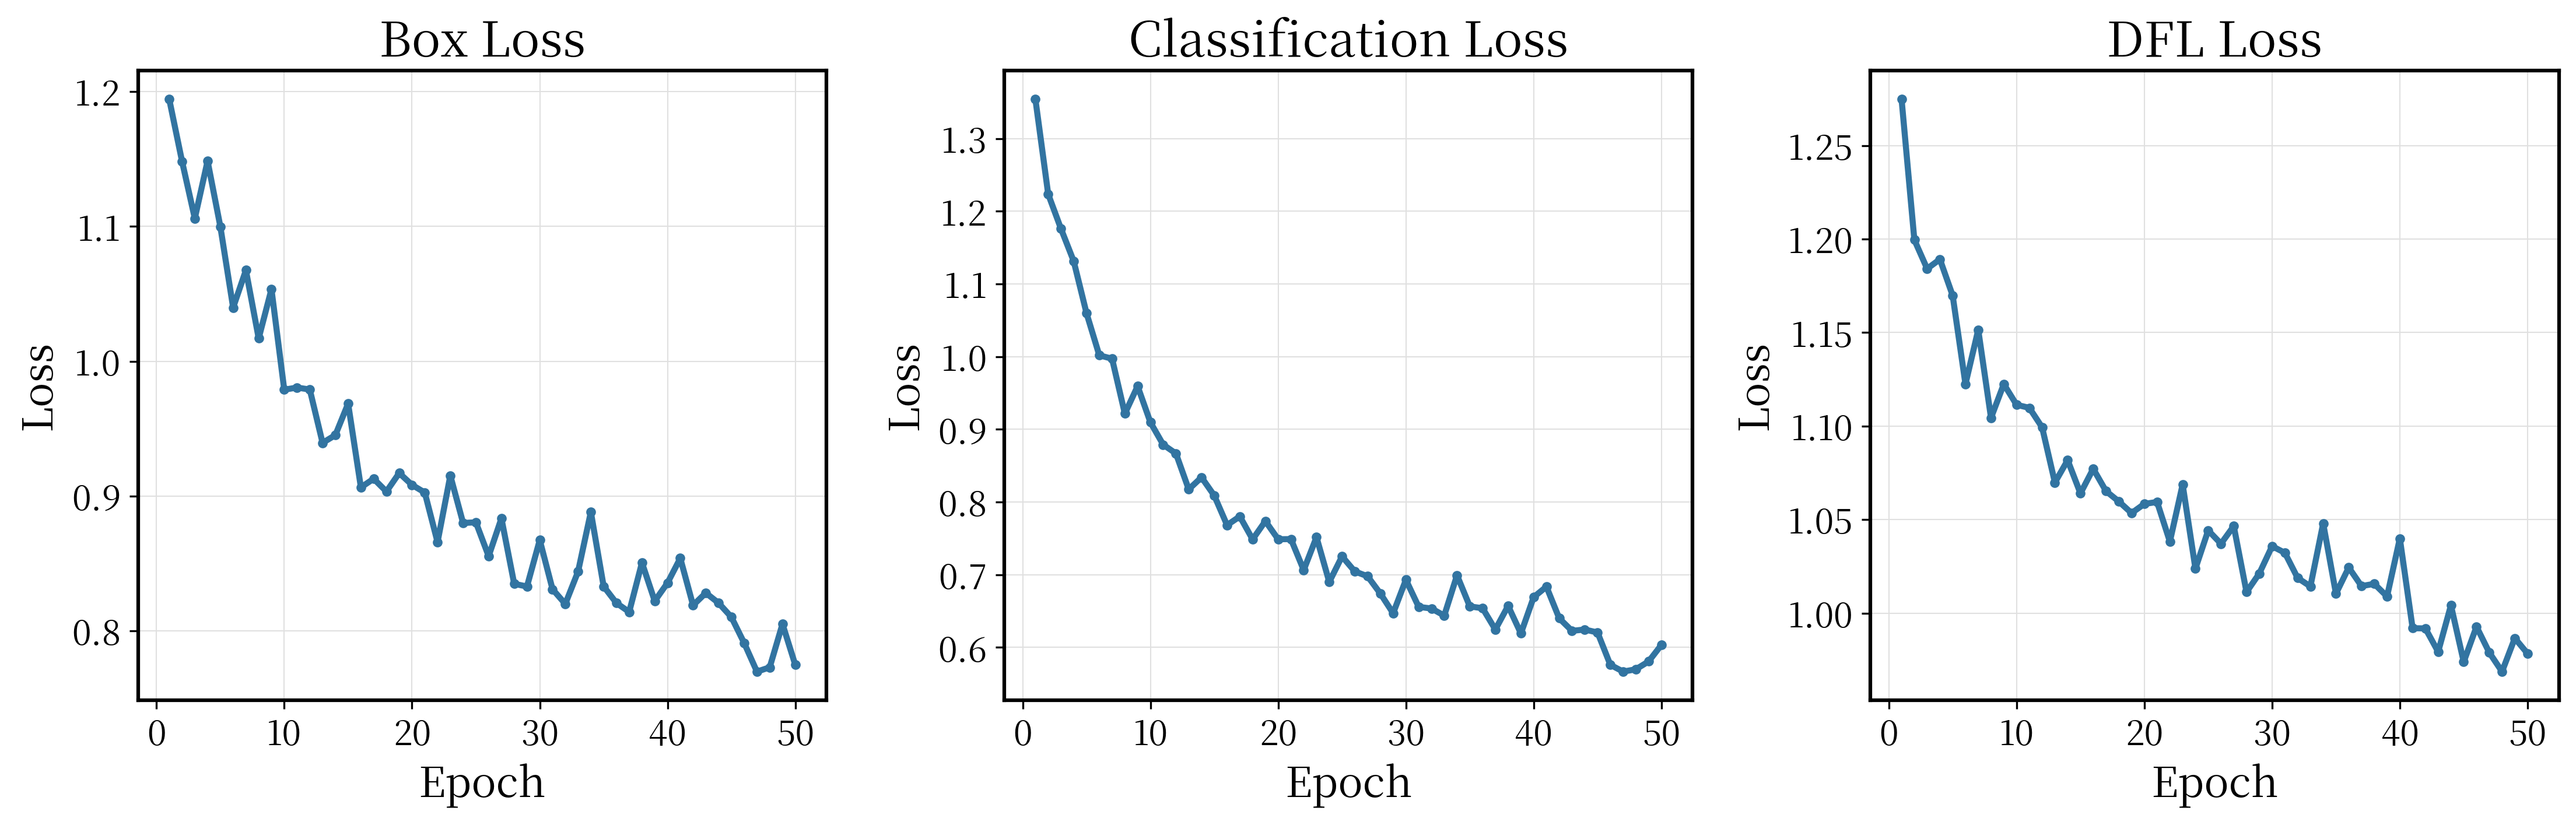
\includegraphics[width=0.8\textwidth]{figs/fig01_train_loss.png}
\caption{训练损失变化曲线：Box Loss（左）、Classification Loss（中）和DFL Loss（右）}
\label{fig:train_loss}
\end{figure}

Box Loss从1.194（epoch 1）下降至0.775（epoch 50），降幅35.1\%，是三个分量中改善最大的。这说明边界框定位是模型在训练初期学习最快的能力——锚框机制提供了良好的初始化，模型只需学习小幅度的偏移修正。

Classification Loss从1.354下降至0.603，降幅55.5\%。分类损失的相对降幅最大，反映了模型在80类目标之间逐步建立了判别特征。但其绝对值始终低于Box Loss，说明在预训练权重的帮助下，分类比定位更"容易"学习——预训练的CSP-Darknet已经具备了区分不同物体的基础视觉特征。

DFL Loss（Distribution Focal Loss）从1.275下降至0.978，降幅仅23.3\%，收敛最慢。DFL用于预测边界框坐标的概率分布而非单一回归值，其优化难度更大，但能提供更精确的定位——这也是mAP@0.5:0.95（高IoU阈值）指标能达到75\%的关键。

\subsubsection{验证集损失与过拟合分析}

\begin{figure}[H]
\centering
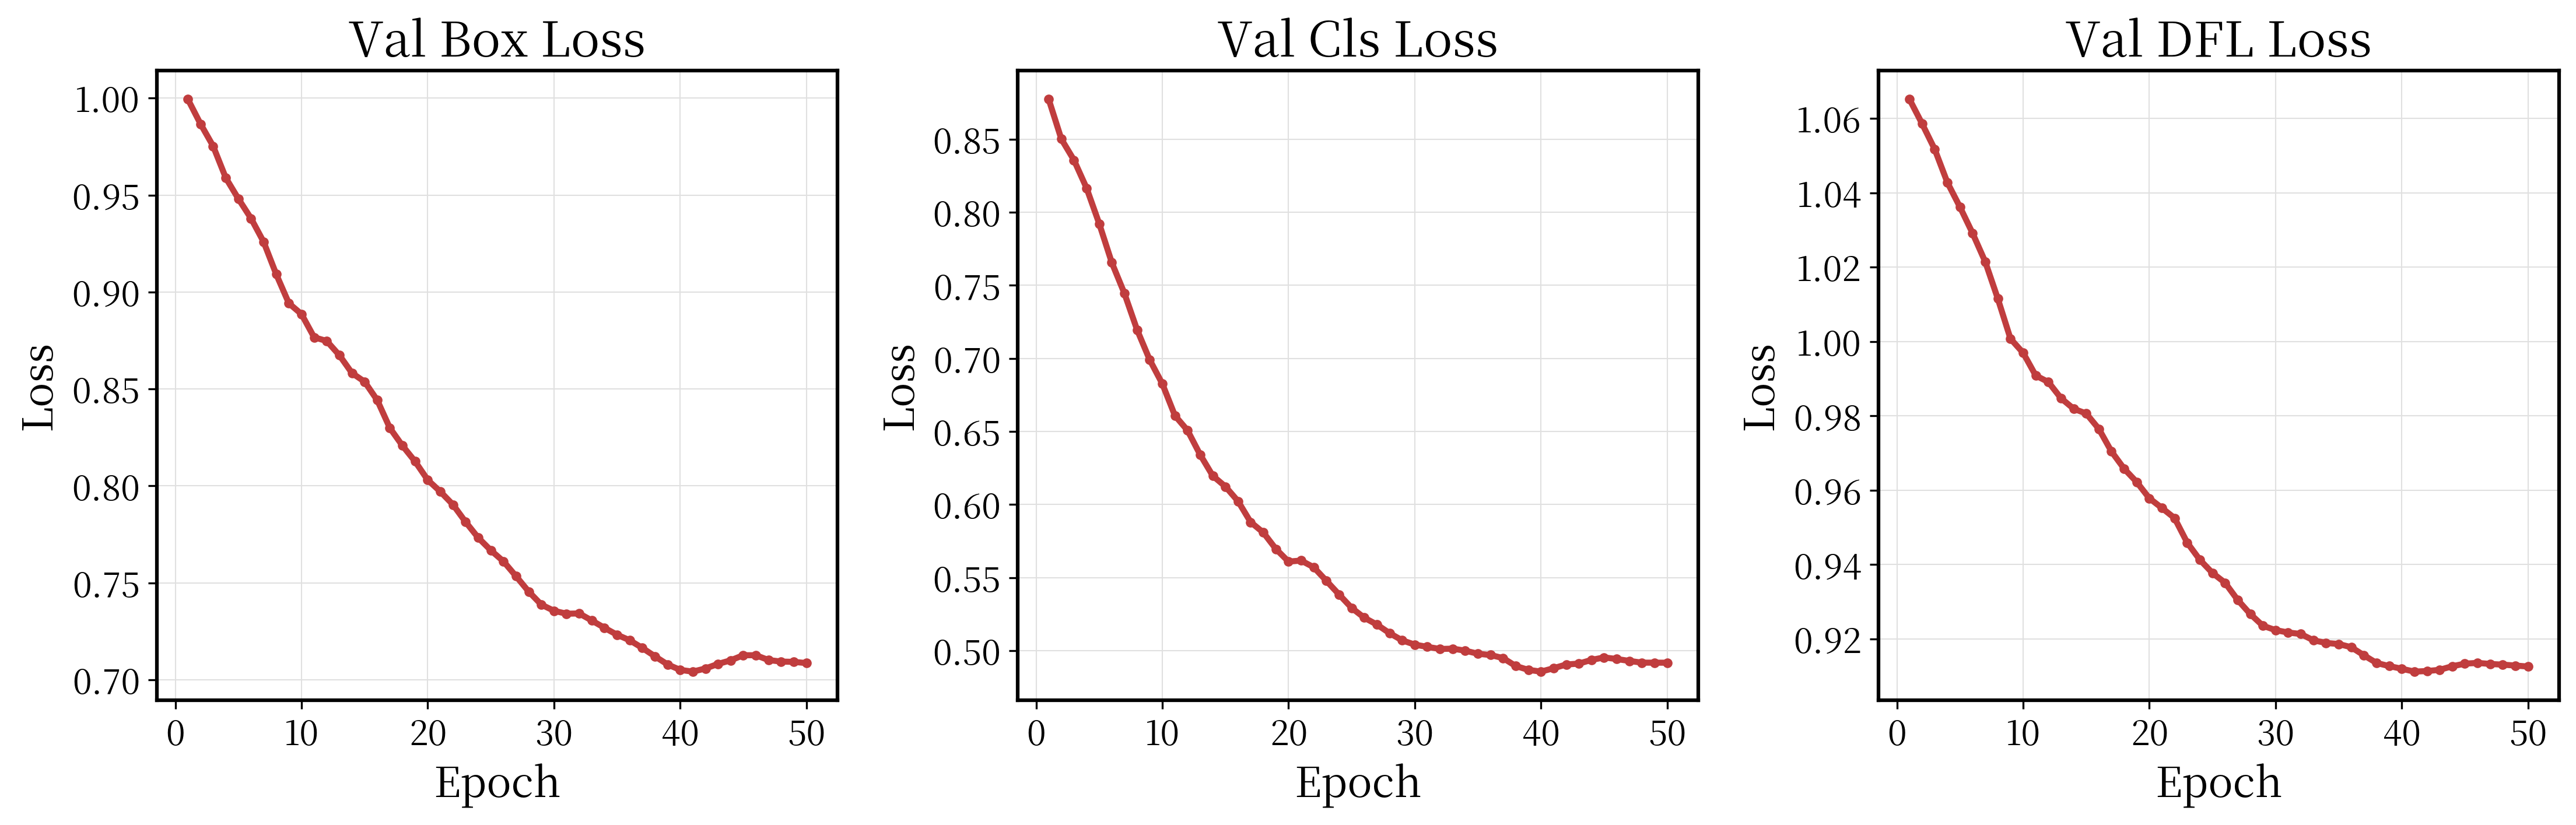
\includegraphics[width=0.8\textwidth]{figs/fig02_val_loss.png}
\caption{验证损失变化曲线}
\label{fig:val_loss}
\end{figure}

图\ref{fig:val_loss}展示了验证集上的损失变化。最终验证损失收敛至box=0.709、cls=0.492、dfl=0.913。由图可以很明显的看出，验证损失始终低于训练损失（验证总损失2.11 vs 训练总损失2.36）。这看似违反直觉，但原因在于训练时Mosaic、随机仿射等增强操作显著增加了学习难度，而验证时不使用这些增强，模型面对的是"更简单"的原始图像。此外，验证损失在后期没有出现上升趋势，说明128张图像虽然很少，但在强数据增强的保护下，模型并未严重过拟合。

\subsubsection{训练阶段划分}

根据各指标的变化规律，50个epoch的训练过程可大致划分为三个阶段：

\begin{table}[H]
\centering
\caption{训练过程三阶段分析}
\label{tab:phases}
\begin{tabular}{lccccc}
\toprule
\textbf{阶段} & \textbf{Epoch} & \textbf{mAP@0.5} & \textbf{Precision} & \textbf{特征} \\
\midrule
快速学习期 & 1--10 & 73.4\%$\to$83.3\% & 69.0\%$\to$85.9\% & 损失急剧下降，基本定位能力形成 \\
稳定改善期 & 10--33 & 83.3\%$\to$90.1\% & 85.9\%$\to$88.6\% & 损失缓慢下降，分类能力精细化 \\
精细收敛期 & 33--50 & 90.1\%$\to$90.4\% & 88.6\%$\to$92.4\% & 损失基本稳定，Precision持续提升 \\
\bottomrule
\end{tabular}
\end{table}

一个有趣的观察是：在第三阶段，mAP@0.5几乎不再提升（仅从90.1\%微升至90.4\%），但Precision从88.6\%跃升至92.4\%。这说明模型在后期并非在“发现更多目标”，而是在“减少误检”——通过更精确的置信度校准，将低质量的检测结果过滤掉。与此同时，Recall在后期从87.9\%（epoch 32峰值）略降至82.4\%，体现了Precision与Recall之间的经典权衡。

\subsection{检测精度分析}

\begin{table}[H]
\centering
\caption{模型最终检测性能与关键里程碑}
\label{tab:final}
\begin{tabular}{lcccc}
\toprule
\textbf{指标} & \textbf{Precision} & \textbf{Recall} & \textbf{mAP@0.5} & \textbf{mAP@0.5:0.95} \\
\midrule
最终值（ep 50） & 92.37\% & 82.38\% & 90.38\% & 75.08\% \\
最佳值 & 93.17\% (ep 45) & 87.87\% (ep 32) & 90.54\% (ep 38) & 75.23\% (ep 40) \\
\midrule
\multicolumn{5}{l}{\textbf{mAP@0.5达标里程碑}} \\
$\geq$80\% &  &  & epoch 7 &  \\
$\geq$85\% &  &  & epoch 15 &  \\
$\geq$90\% &  &  & epoch 33 &  \\
\bottomrule
\end{tabular}
\end{table}

图\ref{fig:map}展示了mAP指标随训练轮次的变化曲线。mAP@0.5从第1个epoch的73.4\%快速上升，仅7个epoch即突破80\%，15个epoch突破85\%，33个epoch突破90\%，最终在第38个epoch达到峰值90.54\%。值得注意的是，模型仅用了约30\%的训练时间（15/50 epoch）就达到了85\%的水平，说明预训练权重提供了极好的初始化，即模型不需要"从零学习"什么是物体，只需微调以适应COCO128的具体数据分布。

mAP@0.5:0.95在第40个epoch达到峰值75.23\%，相比mAP@0.5低了约15个百分点。这一差距的含义是：模型能够较好地检测到目标（IoU$\geq$0.5即算正确），但在精确定位上（IoU$\geq$0.75甚至0.9）仍有提升空间。

\begin{figure}[H]
\centering
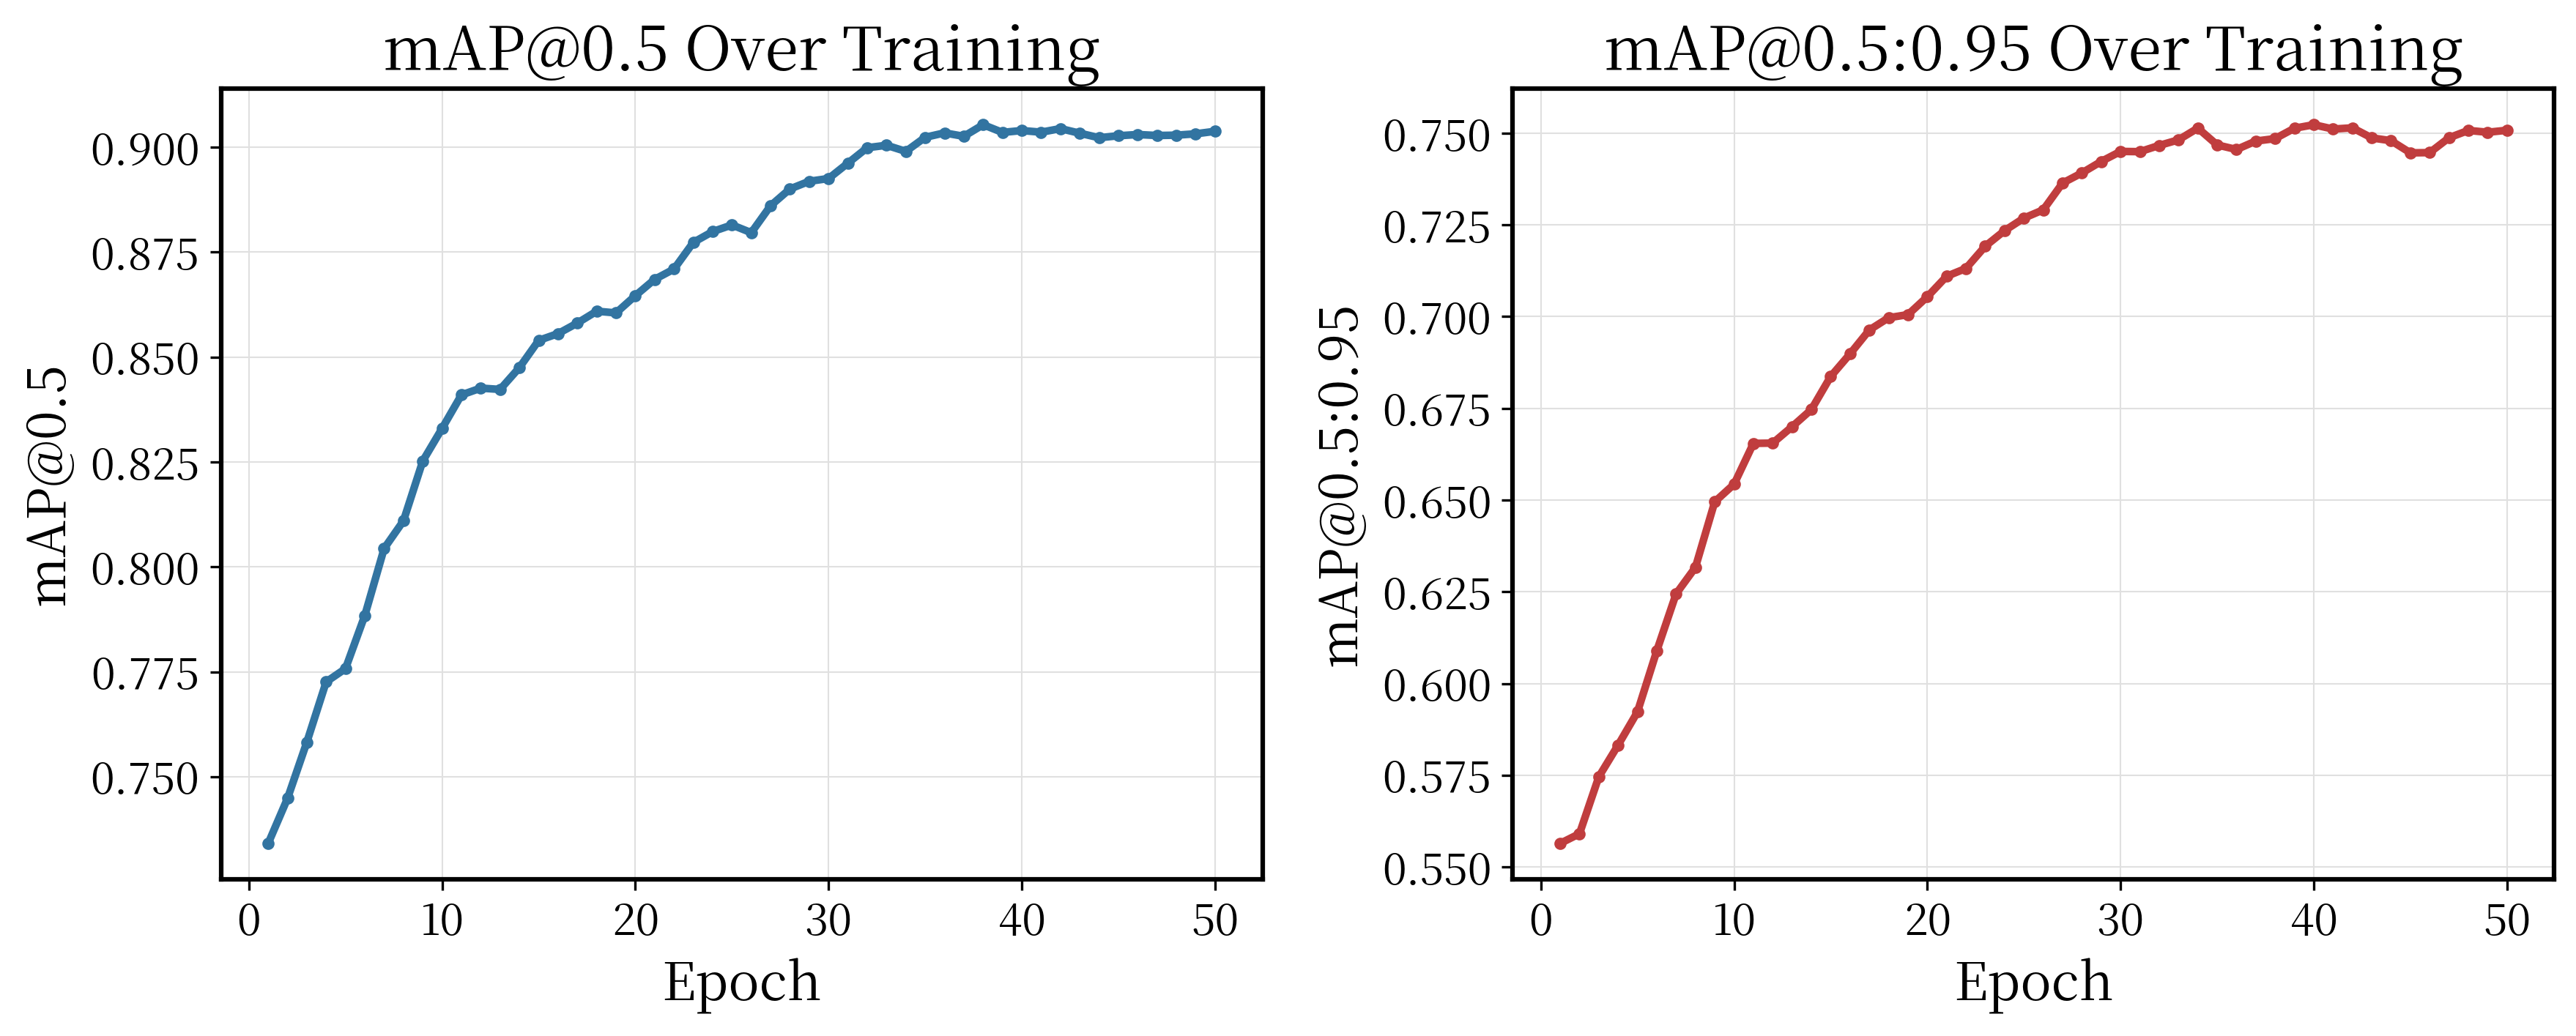
\includegraphics[width=0.8\textwidth]{figs/fig03_map_curves.png}
\caption{mAP@0.5（左）与mAP@0.5:0.95（右）变化曲线}
\label{fig:map}
\end{figure}

图\ref{fig:pr}展示了Precision与Recall的变化曲线。两者在epoch 32附近出现"交叉"：此前Recall上升更快（模型不断发现更多目标），此后Precision上升更快而Recall略有下降（模型开始"精选"高质量检测结果）。最终Precision=92.37\%、Recall=82.38\%，两者存在约10个百分点的差距，说明模型整体偏向于“宁可漏检、不愿误检”的保守策略。在实际自动驾驶等安全关键场景中，可以通过降低置信度阈值来提升Recall，代价是Precision会下降。

\begin{figure}[H]
\centering
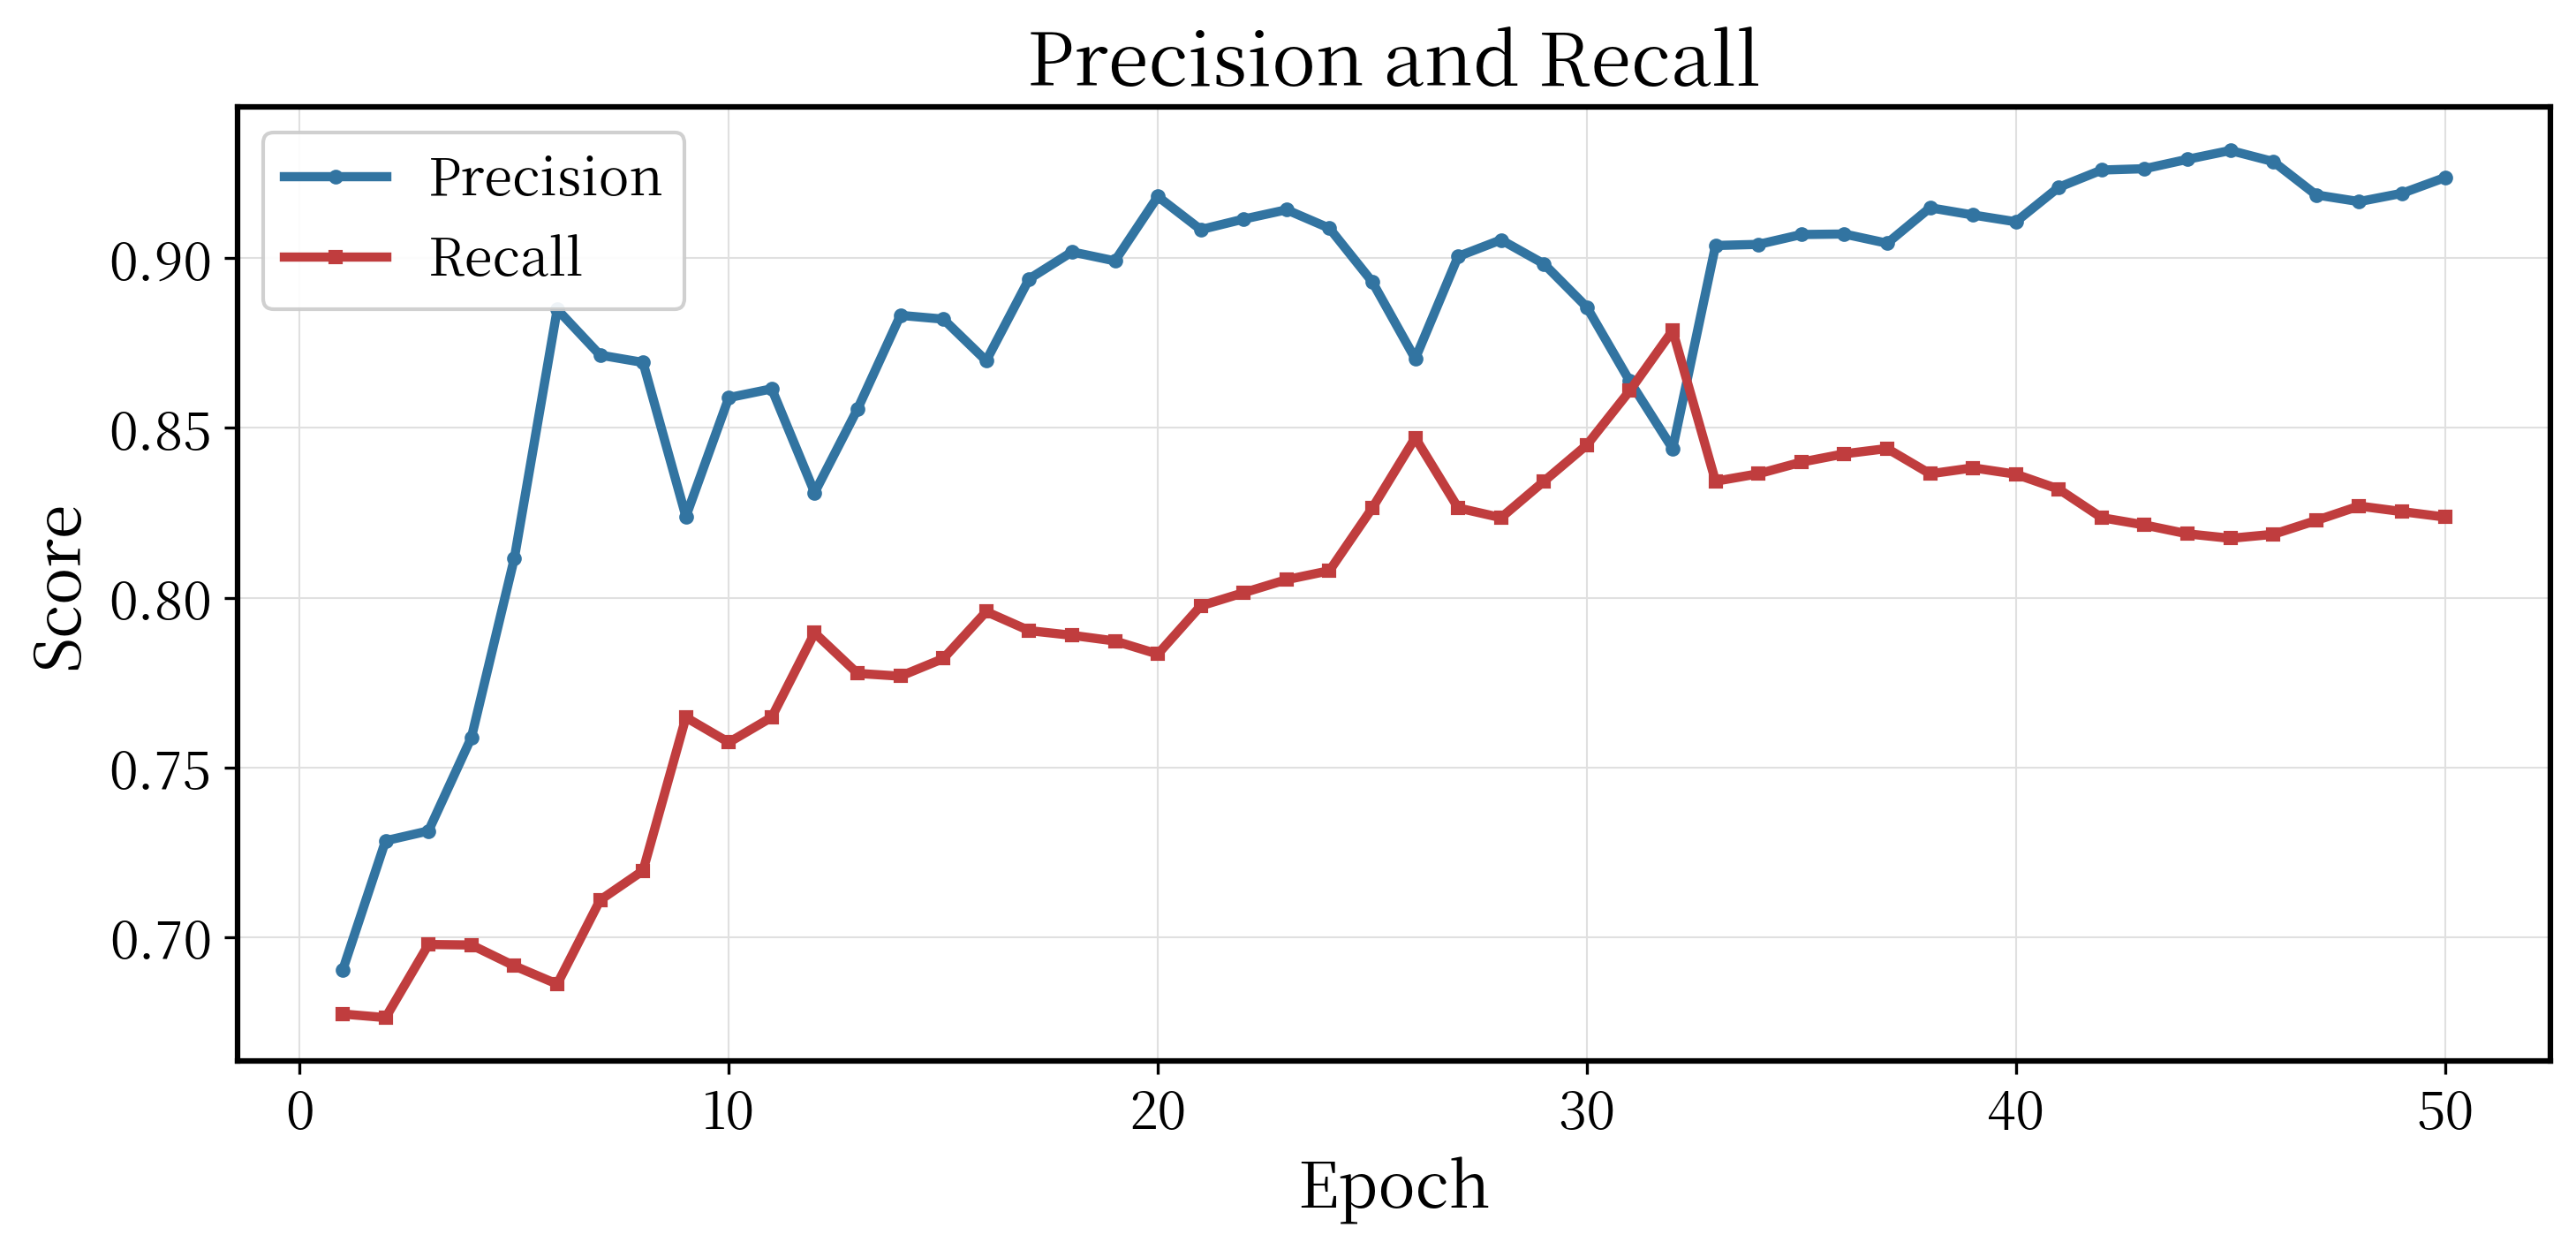
\includegraphics[width=0.8\textwidth]{figs/fig04_precision_recall.png}
\caption{Precision与Recall变化曲线}
\label{fig:pr}
\end{figure}

\subsection{学习率与总损失}

图\ref{fig:lr}展示了学习率调度策略。Warmup阶段（前3个epoch）学习率从接近零线性增长至峰值，随后按余弦函数平滑衰减。这种调度方式有两个优势：（1）Warmup阶段避免了训练初期因大学习率导致的参数剧烈震荡，尤其在使用预训练权重时，过大的初始更新可能破坏已有的特征表示；（2）余弦衰减相比阶梯式衰减更加平滑，避免了学习率突变时loss的瞬时跳升。

\begin{figure}[H]
\centering
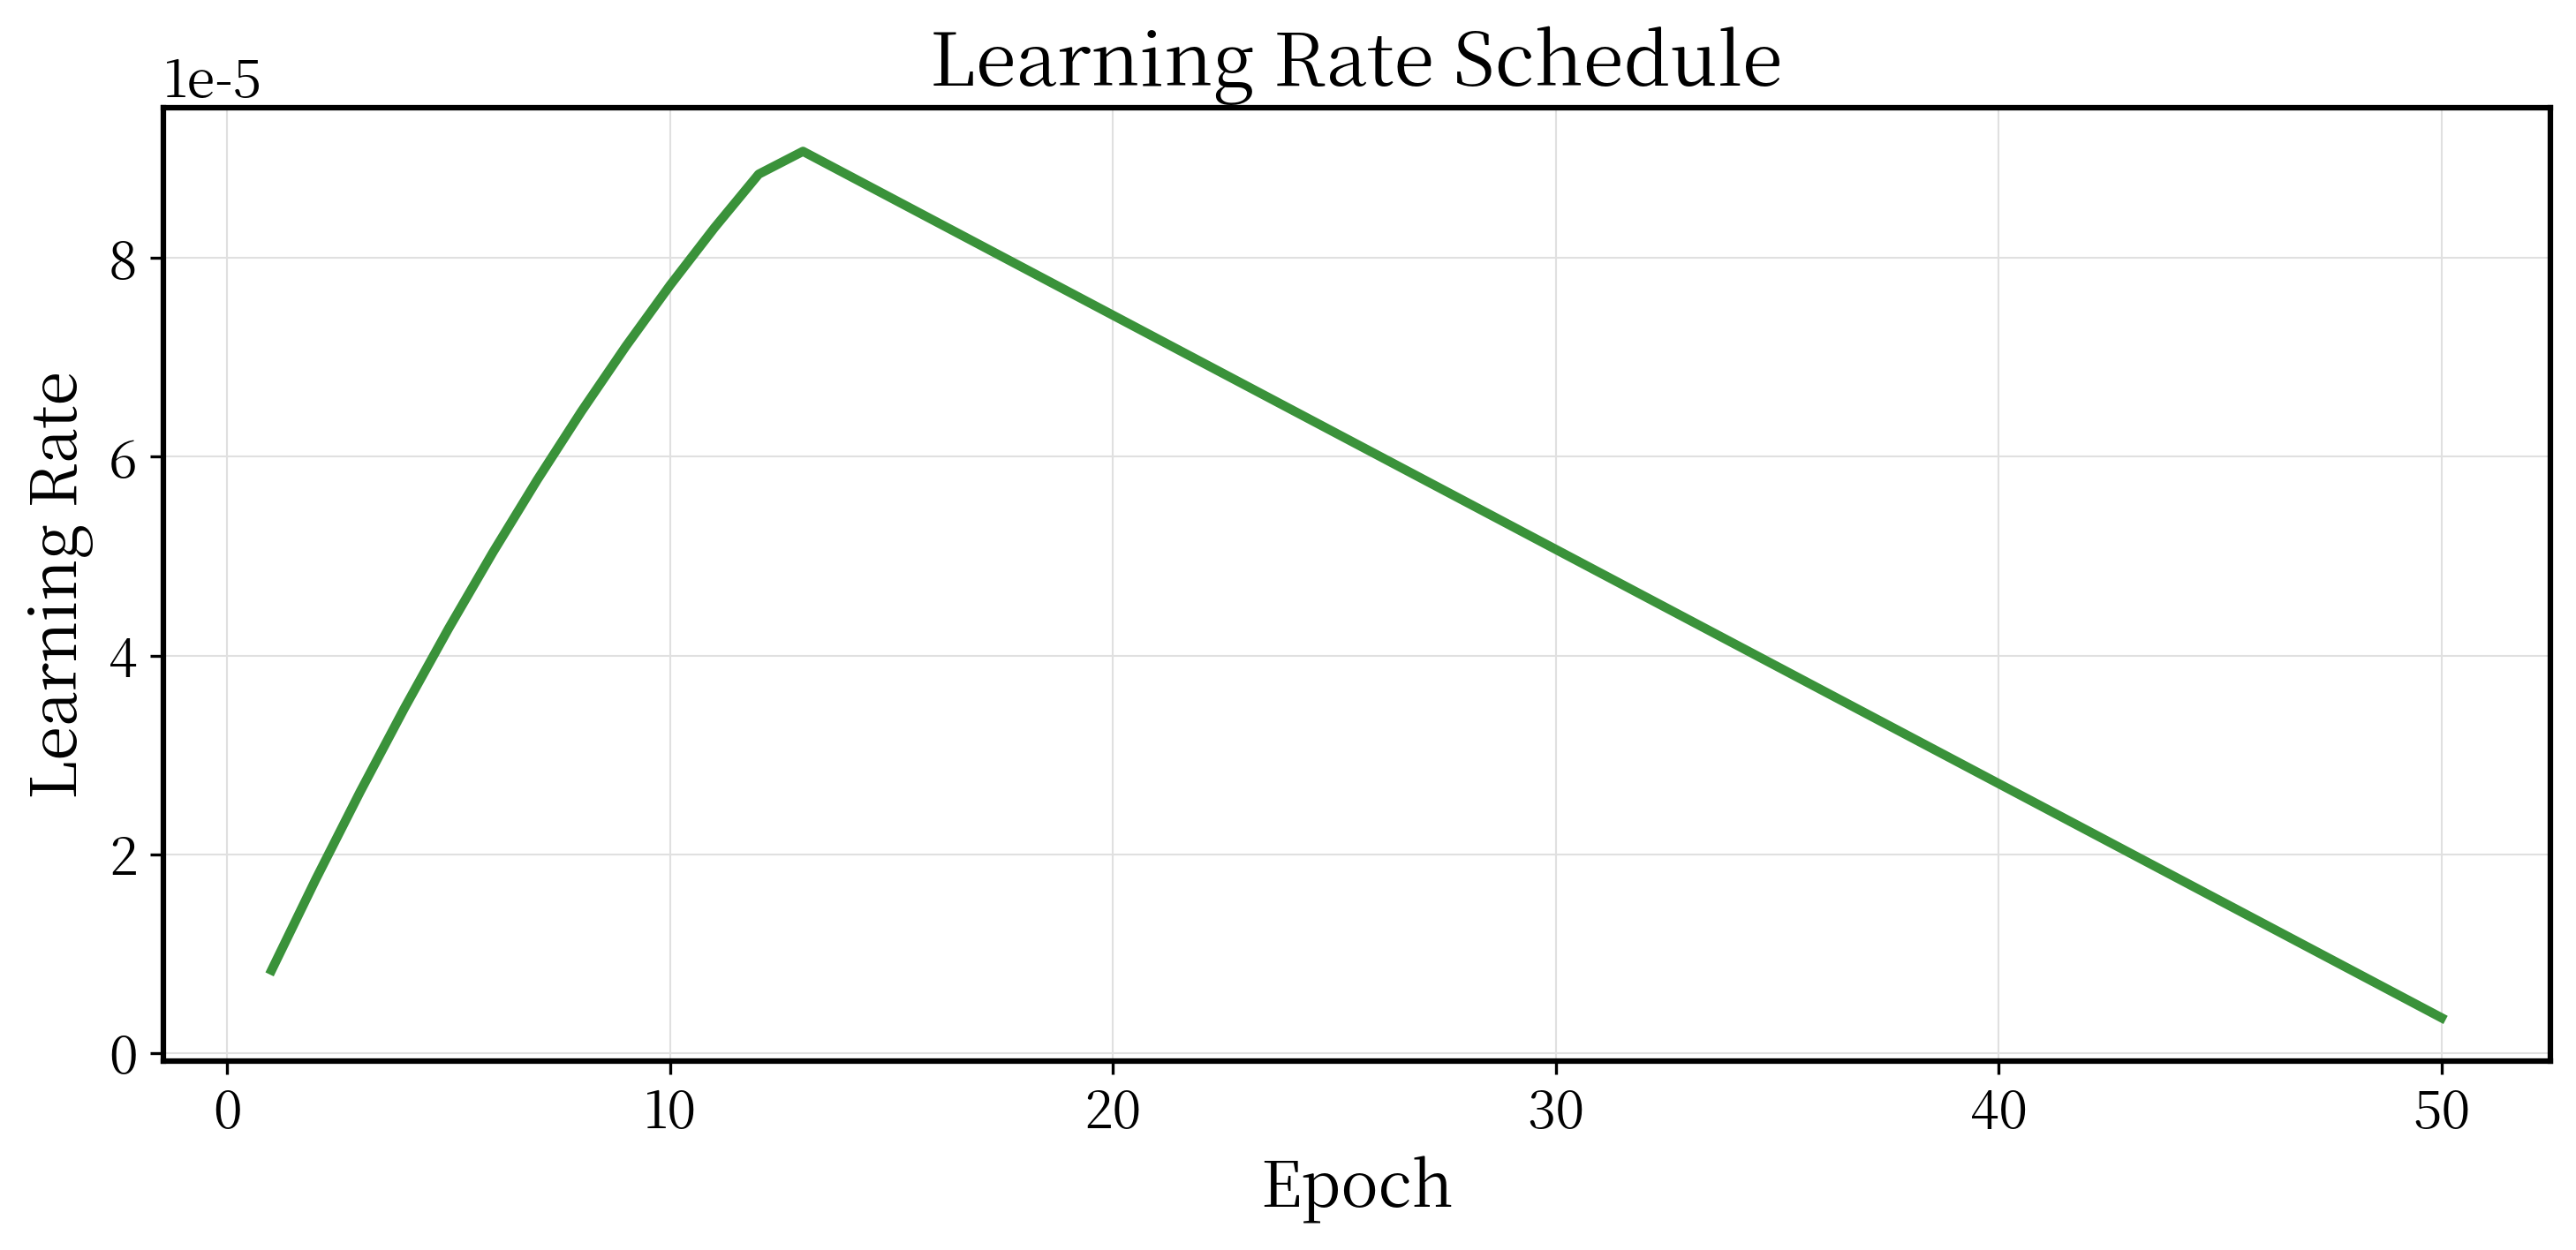
\includegraphics[width=0.8\textwidth]{figs/fig05_lr.png}
\caption{学习率调度曲线}
\label{fig:lr}
\end{figure}

图\ref{fig:summary}将所有关键指标汇总展示。从中可以更直观地看出各指标的收敛节奏差异：Precision和mAP在前20个epoch改善最快（分别从69\%升至92\%、从73\%升至86\%），后30个epoch主要起精细打磨的作用。

\begin{figure}[H]
\centering

\includegraphics[width=0.8\textwidth]{figs/fig06_summary.png}
\caption{训练指标汇总}
\label{fig:summary}
\end{figure}

图\ref{fig:total_loss}展示了训练与验证总损失的对比。训练总损失从3.82（epoch 1）下降至2.36（epoch 50），验证总损失从2.94下降至2.11。两者之间的间隔从初始的0.88缩小至0.25，说明模型在训练过程中逐渐弥合了训练与验证之间的差距。第40个epoch附近（Close Mosaic生效后），训练损失出现短暂的下降加速，因为模型不再面对Mosaic合成图像的额外难度。

\begin{figure}[H]
\centering
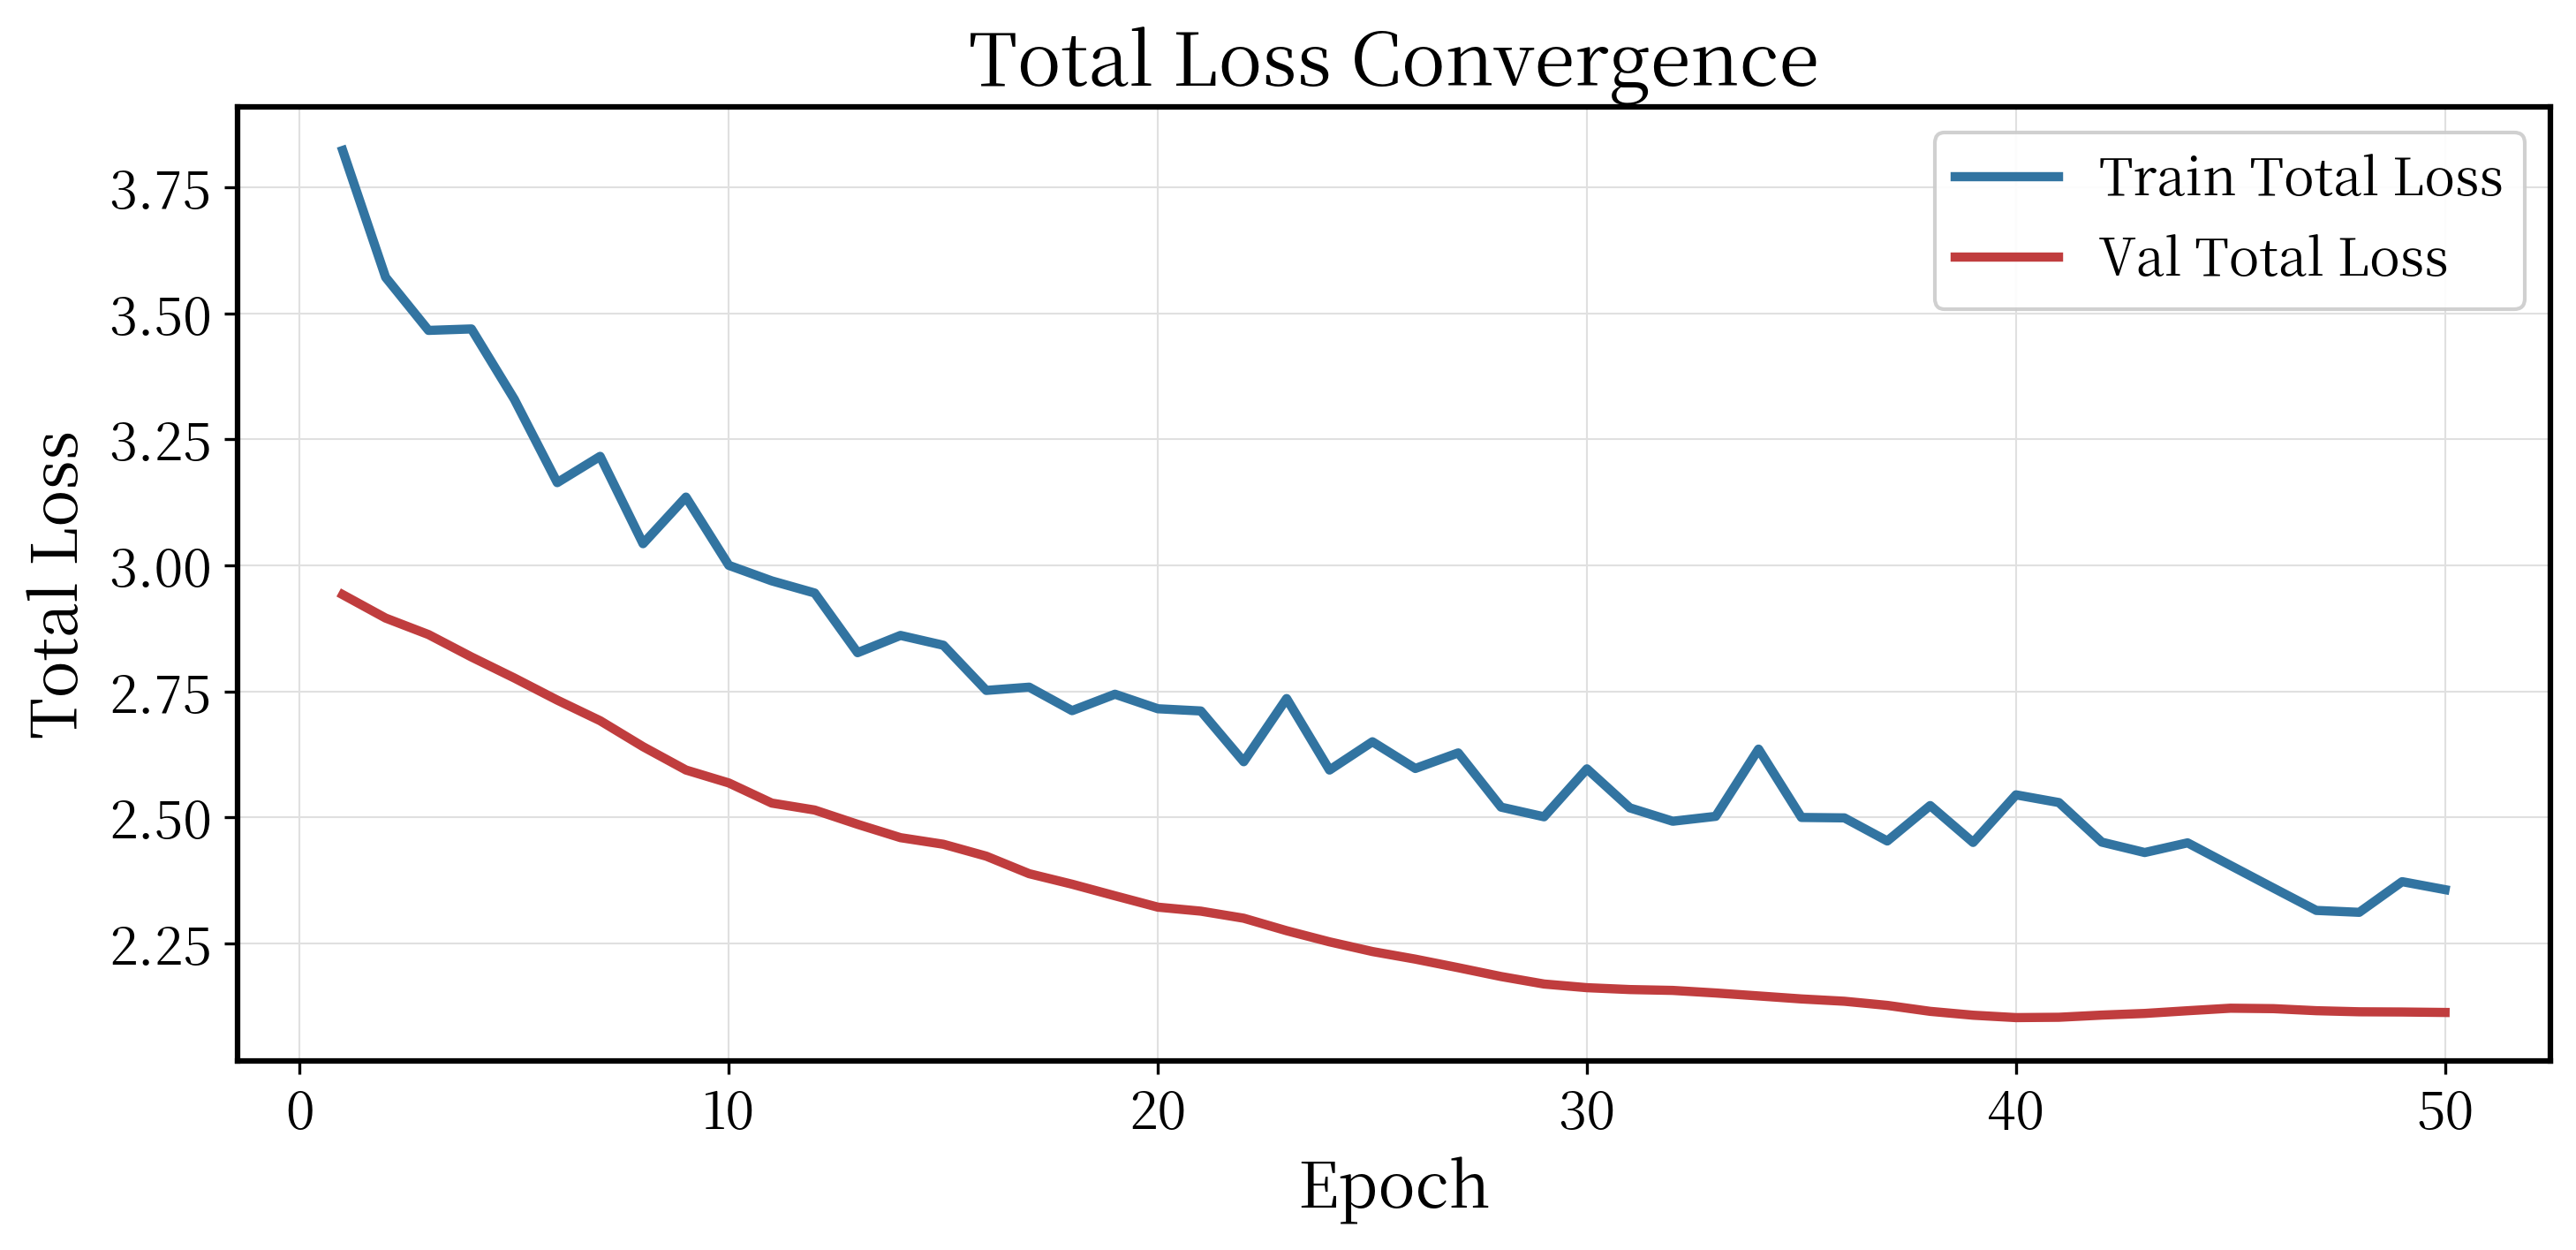
\includegraphics[width=0.8\textwidth]{figs/fig07_total_loss.png}
\caption{训练与验证总损失变化曲线}
\label{fig:total_loss}
\end{figure}

\subsection{检测样例分析}

为了直观评估模型的检测能力，我们在两张标准测试图像上进行了推理，检测结果如表\ref{tab:detect}所示。

\begin{table}[H]
\centering
\caption{样例图像检测结果}
\label{tab:detect}
\begin{tabular}{llccc}
\toprule
\textbf{图像} & \textbf{检测类别} & \textbf{数量} & \textbf{置信度范围} & \textbf{特点} \\
\midrule
\multirow{2}{*}{bus.jpg} & person & 4 & 0.58--0.89 & 远近不同尺度的行人 \\
 & bus & 1 & 0.85 & 大面积目标 \\
\midrule
\multirow{3}{*}{zidane.jpg} & person & 2 & 0.85--0.88 & 主体人物 \\
 & tie & 1 & 0.64 & 中等目标 \\
 & cell phone & 1 & 0.28 & 小目标，置信度较低 \\
\bottomrule
\end{tabular}
\end{table}

可以从如下角度分析检测结果：

（1）多尺度检测能力：bus.jpg中，4个行人分布在不同距离（近处大目标置信度0.89，远处小目标置信度0.58），模型均能成功检测，说明FPN-PAN的多尺度特征融合机制有效发挥了作用。

（2）小目标检测的挑战：zidane.jpg中的手机（cell phone）置信度仅0.28，远低于其他目标。这反映了小目标检测的固有难度：手机在图像中仅占极少的像素，经过多次下采样后特征极度稀疏。在实际应用中，0.28的置信度可能不会通过默认的0.25阈值筛选，或者在NMS过程中被更高置信度的框抑制。

（3）类别语义理解：模型不仅检测到了人和车这样的常见目标，还识别出了领带和手机这类小而隐蔽的物体，说明在预训练权重的帮助下，模型已经具备了较为丰富的视觉语义理解能力。

% ==============================================================
\section{深入讨论}
% ==============================================================

\subsection{为什么128张图像就能训练出90\%+的检测器？}

COCO128仅有128张图像，但模型达到了mAP@0.5=90.4\%。这一结果的关键在于迁移学习与数据增强的协同效应。

迁移学习方面，模型从在完整COCO数据集（约33万张图像）上预训练的权重出发，427个权重层全部成功迁移。这意味着模型已经"知道"什么是物体、如何提取边缘和纹理特征，微调仅需调整高层特征以适应COCO128的数据分布。如果从随机初始化开始训练，128张图像远不足以学习有意义的特征表示。

数据增强方面，Mosaic增强在每个epoch中相当于将128张图像扩展为不同的4图组合，理论上可以产生$C_{128}^{4} \approx 1.1 \times 10^7$种不同的训练样本。加上随机仿射和HSV抖动，模型在50个epoch中几乎不会看到完全相同的训练样本，有效缓解了过拟合。

\subsection{三种IoU损失的对比}

CIoU损失是Box Loss取得35\%降幅的重要因素。三种IoU变体的对比如下：

\textbf{IoU Loss}：$\mathcal{L} = 1 - IoU$。致命缺陷：当预测框与真实框不相交时，$IoU=0$，梯度为零，无法指导优化方向。

\textbf{GIoU Loss}：引入最小外接矩形的面积差，解决了不相交时的梯度问题。但GIoU只关注重叠面积，不直接惩罚中心点偏离，收敛较慢。

\textbf{CIoU Loss}：在GIoU基础上增加了中心点距离惩罚项$\frac{\rho^2}{c^2}$和宽高比一致性约束$\alpha v$。这使得优化同时从三个维度推动预测框向真实框靠拢：增大重叠、缩小中心距离、对齐宽高比。

从实验数据来看，Box Loss在前10个epoch就从1.194下降至0.979（降幅18\%），而后40个epoch仅继续下降至0.775（降幅21\%），说明CIoU的多维优化在训练初期就快速"粗对齐"了预测框，后期则进行精细调整。

\subsection{Precision-Recall权衡与阈值选择}

最终模型的Precision（92.4\%）显著高于Recall（82.4\%），这反映了默认置信度阈值（0.25）下模型的行为偏好。在实际应用中，这一权衡需要根据场景调整：

在自动驾驶中，漏检行人（低Recall）的代价远大于误检路灯（低Precision），因此应降低阈值以提高Recall；在工业质检中，误报会导致大量正常品被剔除（高成本），因此应提高阈值以保证Precision。本实验中mAP@0.5同时评估了所有可能阈值下的综合性能，因此90.4\%的mAP意味着在大多数阈值设定下模型都能保持较好的检测质量。

% ==============================================================
\section{实验总结}
% ==============================================================

本实验在COCO128数据集上训练了YOLOv5s目标检测模型，经过50个epoch的训练，达到了mAP@0.5=90.4\%、Precision=92.4\%、mAP@0.5:0.95=75.1\%的检测性能，满足实验要求的90\%精度标准。

通过实验，可以得到如下结论：

（1）多任务联合优化。目标检测的三个子任务——定位（Box Loss）、检测（Obj Loss）和分类（Cls Loss）——具有不同的学习速度和优化难度。Box Loss因锚框初始化而下降最快，Cls Loss因预训练特征而绝对值最低，DFL Loss因其分布预测的本质而收敛最慢。

（2）数据增强对小数据集至关重要。128张图像在Mosaic + 仿射 + HSV增强的保护下，模型未出现严重过拟合（验证loss持续下降或稳定）。Close Mosaic机制在最后10个epoch关闭增强，使模型最终适配真实图像分布。

（3）预训练权重与微调的关系。模型仅需7个epoch即突破mAP@0.5=80\%，体现了迁移学习的巨大价值——预训练权重提供了通用的视觉特征，微调仅需学习任务特定的检测头参数和少量的特征适配。

（4）多尺度检测的必要性。从检测样例可以看出，同一图像中的目标尺度可以跨越数倍甚至数十倍。FPN-PAN的三尺度检测头设计（$80\times80$、$40\times40$、$20\times20$）是在这种场景下保持高检测率的关键。

\begin{sloppypar}
本实验代码位于：\url{https://github.com/neverwinHao/deep-learning-project/tree/main/Exp5/code}
\end{sloppypar}

\end{document}
